
\chapter{Changements de phases des corps purs}

Un corps pur est un corps composé d'une seule espèce chimique. Ce corps peut prendre trois états : solide, liquide et gaz.\\

Lorsqu'on a un changement d'état, ou une transition de phase, on a une modification de l'ensemble des propriétés physiques, mécaniques et chmiques de notre système.\\

Schématiquement, l'ensemble des trasitions de phases peut se représenter ainsi :

\begin{figure}[H]
\centering
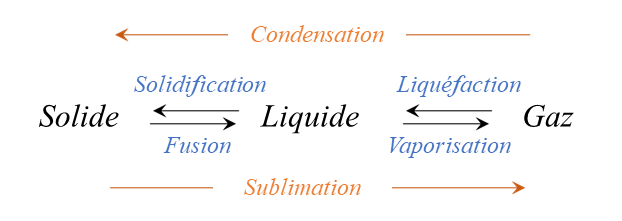
\includegraphics[scale=0.5]{C5F1.PNG}
\caption{Changements de phases}
\end{figure}

\section{Chaleur latente de changement d'état}

Au cours d'un changement de phase, la transformation s'effectuant est par définition \textbf{isobare} et \textbf{isotherme}. 

\begin{definition}[Chaleur latente]

La chaleur latente correspond à la chaleur nécessaire au changement d'état d'un corps passant d'une phase 1 à une phase 2. Notée $\mathcal{L}$, on la retrouve le plus souevnt exprimée pour une mole. On a alors

\begin{equation}
L_{m_{1\rightarrow2}}=\frac{Q_p}{n}~~~~~~~~[L_m]=J.mol^{-1}
\end{equation}
\end{definition}

Or, nous sommes à pression et température constante, donc
$$L_{m_{1\rightarrow2}}=\Delta_rH_{m_{1\rightarrow 2}} \simeq \Delta_rH_{m_{1\rightarrow 2}}^0$$r

On considère notre changement d'état comme un équilibre thermodynamique, on peut donc écrire 
$$\Delta_rG = \Delta_rH _ T\Delta_rS =0$$
Soit
$$\Delta_rH = T \Delta_rS \Leftrightarrow \Delta_rS = \frac{\Delta_rH}{T}=\frac{L_m}{T}$$
On sait que la différentielle de l'entropie s'écrit telle que
$$dS=\left ( \frac{\partial S}{\partial T}\right ) _V dT + \left ( \frac{\partial S}{\partial V}\right ) _T dV$$
Ici, notre température est constante, donc $dT=0$, on en déduit que
$$dS = \left ( \frac{\partial S}{\partial V}\right ) _T dV$$

D'autres part, on sait que 
$$dU = -PdV + TdS$$
$$dH = VdP+TdS$$
$$dG=VdP-SdT$$
$$dF=-PdV-SdT$$

On en déduit les relations de Maxwell\footnote{A ne surtout pas confondre avec les équations de Maxwell qui correspondent à des relation en électromagnétisme}.

\begin{theorem}[Relations de Maxwell]
Les relations de Maxwelle sont des équations aux dérivées partielles permettant de mettre en lien les différentes fonctions et variables d'état. Ainsi, on a

\begin{equation}
 \left ( \frac{\partial P}{\partial S}\right ) _V =  \left ( \frac{\partial T}{\partial V}\right ) _S \textrm{   ;   } \left ( \frac{\partial V}{\partial S}\right ) _P =  \left ( \frac{\partial T}{\partial P}\right ) _S
 \end{equation}
  \begin{equation}
 \left ( \frac{\partial V}{\partial T}\right ) _P = - \left ( \frac{\partial S}{\partial P}\right ) _T \textrm{   ;   } \left ( \frac{\partial P}{\partial T}\right ) _V =  \left ( \frac{\partial S}{\partial V}\right ) _T
 \end{equation}
 
 \end{theorem}
 
 A partir de l'ensemble de ces relations, nous allons pouvoir en déduire
 $$dS=\left ( \frac{\partial S}{\partial V}\right ) _TdV=\left ( \frac{\partial S}{\partial V}\right ) _TdV$$
 On trouve ainsi que
 $$\frac{dP}{dT}\simeq\frac{dS}{dV} \simeq \frac{_Delta S}{\Delta V}$$
 Finalement, on a
 $$\Delta S = \Delta V  \left ( \frac{d P}{d T}\right ) = \frac{\Delta H}{T}$$
 Soit la relation
 \begin{equation}
 \Delta H_{1\rightarrow2} = \Delta V_{1\rightarrow2} T_{1\rightarrow2} .\left ( \frac{d P}{d T}\right ) 
 \end{equation}
 
 Dans le cadre d'une transformation gaz vers liquide, onle volume de gaz étant nettement supérieur au volume de liquide, on a $\Delta V \simeq V_g =\frac{RT}{P}$ pour une mole. On trouve alors
 \begin{equation}
 \Delta H_{1\rightarrow2} = \frac{RT^2}{P} \left ( \frac{dP}{dT} \right )
 \end{equation}
 
On aurait ou déduire le même résultat à aprtir de la \textbf {Relation de Clapeyron}.
 
 \begin{theorem}[Relation de Clapeyron]
 A température $T$ donnée d'un changement d'état allant d'une phase 1 à ue phase 2, on a
 \begin{equation}
 \left ( \frac{dP_{1\rightarrow2}}{dT} \right ) = \frac{\Delta H_{1\rightarrow2}}{T \Delta V _{1\rightarrow2}}
 \end{equation}
 \end{theorem}
 
 \begin{remark}
 On notera que les enthalpies étant souvant molaires, on aura un volume molaire au dénominateur de notre quotient.
 \end{remark}
 
 \section{Equilibre à l'interface liquide-gaz}
 
 On représente le diagramme à température constante suivant, représentant les variation de pression et de volume au cours d'un changement de phase.\\
 
 \begin{figure}[H]
 \centering
 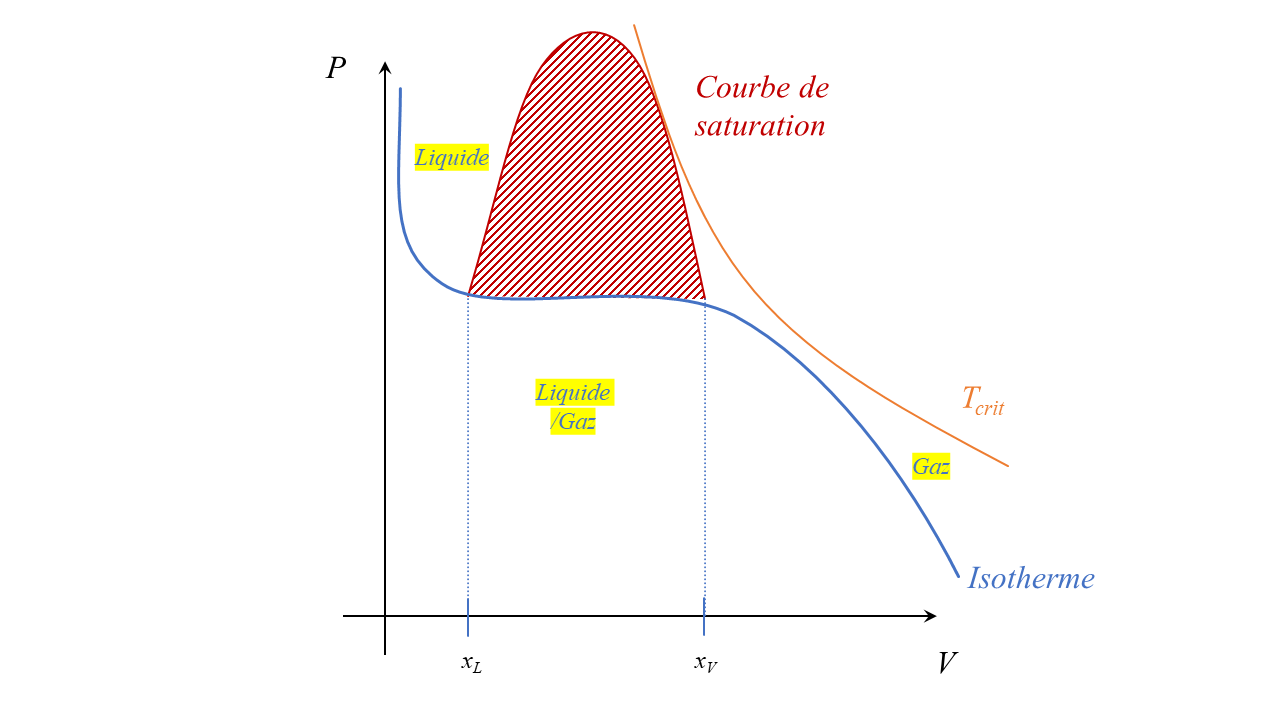
\includegraphics[scale=0.5]{C5F2.PNG}
 \caption{Courbe de stauration et plateau de changement de phase dans un diagramme $(P,V)$}
 \end{figure}
 
 On peut ici voir notre courbe de saturation correspondant pour son extrémité gauche au début de l'ébullition de notre liquide (appelée \textbf{courbe d'ébullition}), et pour son extrémité droite la vaporisation de note corps (appelée \textbf{courbe de rosée}).\\
 
 On peut ici utilir un théorème appelé théorème des moments.\\
 
 \begin{theorem}[Théorème des moments]
 Si on prend un point $M$ situé sur l'isotherme, entre $x_L$ et $x_V$, et deux points $A$ et $B$ correspondant aux extrema de notre transformations, on a 
 \begin{equation}
 m_L . \overline{AM} = m_V.\overline{MB}
 \end{equation}
 On peut réecrire cette équation sous la forme
 \begin{equation}
 (1-x_V)\overline{AM}=x_V\overline{MB}
 \end{equation}
 Avec $x_V = \frac{m_V}{m_L+m_V}$
 \end{theorem}
 
 Pour finir, on peut définir un point spécifique de notre courbe correspondant au sommet de la courbe de saturation et appelé le \textbf{point critique}.\\
 
 \begin{definition}[Point critique]
 Le point critique correspond au poit à partir duquel il n'y a plus de palier de changement de phase. Ainsi, notre corps pour des pressions ou températures supérieures ou égales se retrouvera dans un état situé entre un état gaz et un état fluide qu'on appelle état \textbf{supercritique}.
 \end{definition}
 
 Pour ce fluide, la hclaeur latente tend vers zéro, on a donc un poit d'inflexion impliquant
 $$\left ( \frac{\partial P}{\partial V}\right ) _{T_c}=\left ( \frac{\partial ^2 P}{\partial V^2} \right ) = 0$$
 
 Si on conbine avec une fonction d'état $f(P,V,T)$, on retrouve $T_c, P_c, V_c$.
 
